\section{Introduction}
\IEEEPARstart{I}{ndustrial} optimization occurs above the regulatory control
layer: engineers adjust recipes, schedules, and setpoints to meet quality,
throughput, energy, or discharge objectives while PLCs and local controllers
retain fast regulation. The supervisory decision, however, is only one part of
the intervention: a usable execution path must also establish who may change
which parameter, which limits are active, whether the device accepted the
command, and whether the process improved. Because these concerns are normally
embedded in
application code, they are rebuilt for every new process, protocol, or agent
framework, and the rebuild is where duplicated drivers, ad-hoc permission
checks, and logs that cannot be tied back to a decision accumulate.

These concerns recur across plants whose physics and objectives differ---
injection molding coupling part weight to pressure, time, and temperature;
wastewater treatment (WWTP) balancing effluent constraints against aeration and
dosing cost; annealing trading material properties against line speed; and
BOPET (biaxially oriented polyethylene terephthalate) coordinating casting and
stretching sections.
All need an auditable bridge from a team-level task to heterogeneous acquisition
and control nodes.

Large language model (LLM) agents are being studied for industrial diagnosis,
engineering assistance, and PLC-program generation
\cite{raza2025industrial,sabetta2025assistant,liu2026agents4plc,fakih2024llm4plc},
including simulated controller and machine interaction
\cite{vyas2026ftc,hofmann2025nlc}. Yet orchestration frameworks and protocol connectivity do not by themselves answer who is authorized, which production limits apply, or how a write is linked to later evidence (Section~\ref{sec:related}). Moreover, a task state such as
\texttt{COMPLETED} can coexist with a missed process objective.

\system{} addresses this execution gap through member--node bindings and shared
line, product, recipe, and run context. Nodes expose engineering quantities
rather than register addresses; bindings scope sanctioned tools; and
intervention records retain the proposal, execution result, observation, and
verdict. Fig.~\ref{fig:intro} contrasts this organization with application-specific integration; fast regulation, certified protection, and the choice of optimization algorithm remain outside the framework.

\begin{figure*}[!t]
\centering
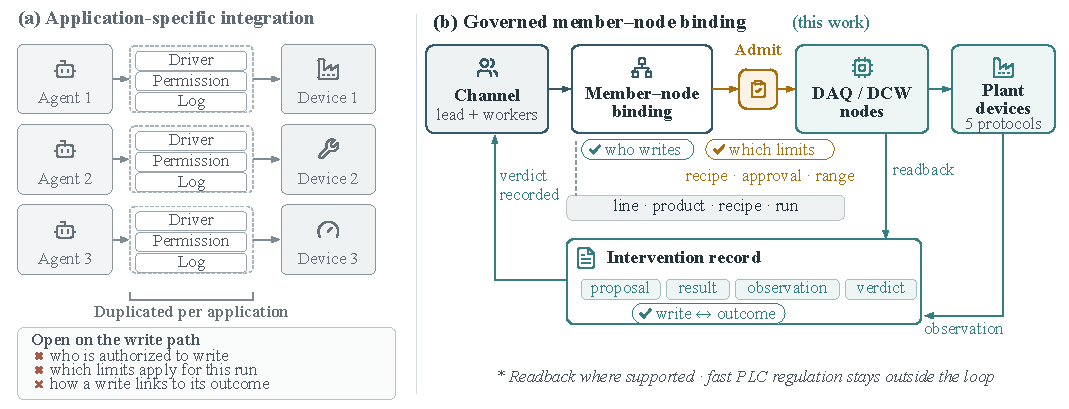
\includegraphics[width=\textwidth]{resources/fig1-governed-binding-v2.pdf}
\caption{Conceptual supervisory integration: (a) application-specific links
duplicating drivers, permissions, and logging per application; (b) governed
member--node binding in \system{}, where requests pass recipe, approval, and
range checks and intervention records return readback, observation, and
verdict. Patterns are compared, not optimization performance; PLC regulation
remains outside the agent-team loop.}
\label{fig:intro}
\end{figure*}

The paper makes four contributions:
\begin{enumerate}
\item a \textbf{capability-based industrial execution architecture} connecting
agent-team identity, semantic data-acquisition (DAQ) and write-control (DCW)
nodes, heterogeneous protocol drivers, and line--product--recipe--run context,
with task membership distinct from physical-write authority;
\item a \textbf{reusable integration boundary} of self-describing node and
driver contracts across five protocol families, versioned production objects,
plugin extension points, and a typed software development kit (SDK), into which
the evaluated reference
adapter projects scenario blueprints while process models and policies remain
external;
\item an \textbf{evidence-preserving governed intervention workflow}
separating admission, optional approval, actuation, readback, observation,
the caller's verdict, compensation, and backstop actions, so a completed task
never stands in for a verified process outcome; and
\item a \textbf{layered evaluation} exercising one governed path through a
mechanism ablation, a deterministic controller, agent-team missions, and
concurrent process missions, with task state and objective attainment reported
separately throughout.
\end{enumerate}
Scope is stated once here and revisited in Section~\ref{sec:limits}: real
software protocol stacks execute against author-implemented dynamic simulators,
scripted policies drive the governed tools for repeatability, and fast
regulation, certified protection, physical-plant transfer, and optimizer
ranking are outside the claims made here.
